% capitulo de implementación
\chapter{Diseño e Implementación}
\section{Arquitectura de la solución}
El siguiente capitulo consta de las bases necesarias para realizar la solución. Esta se compone de 2 elementos principales. 
\begin{itemize}
\item Servidor: Encargado de recodificar (si es necesario) la fuente de audio o video y segmentarla para su distribución.
\item Cliente: Aplicación ejecutada en iOS, encargada de comunicarse al servidor para pedir el flujo de video y entregar información en twitter.
\end{itemize}
% poner figura aqui
La figura presenta una idea general del sistema.\\

\begin{figure}[h!]
	\centering
	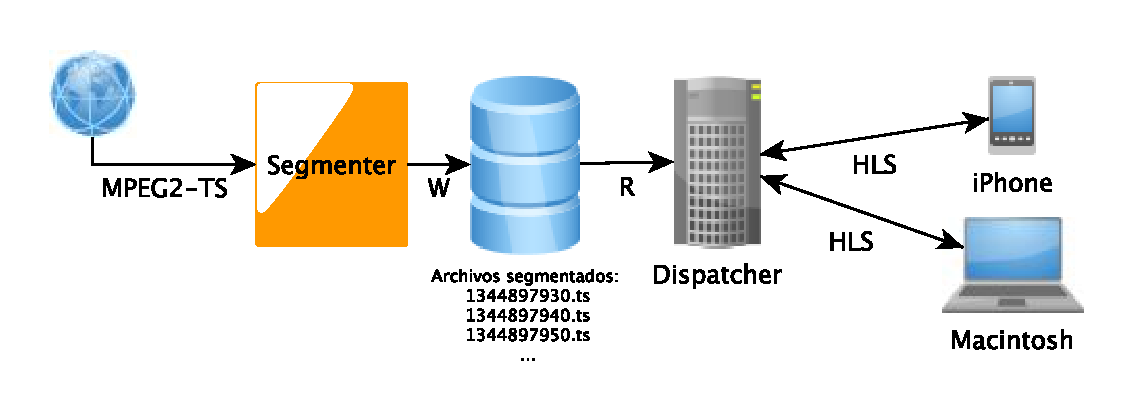
\includegraphics[scale=0.8]{imgs/diagrama_general.eps}
	\caption{Diagrama general de la solución}
	\label{diagramaGral}	
\end{figure}

Respecto a los elementos principales, estos se componen de distintos modulos que serán explicados con más detalle a lo largo del capítulo. Del diagrama se explican de forma general:
\begin{itemize}
\item Segmenter: es una aplicacion que recibe como entrada un flujo de audio y/o video encapsulado en MPEG2-Transport Stream, para luego segmentar el contenido en archivos segmentados de menor duración, estos se guardan en el sistema de archivos del servidor.
\item Dispatcher: Este es un programa dedicado a recibir peticiones de los clientes, para entregar un flujo de video mediante el protocolo HTTP Live Streaming.
\item iPhone y Macintosh: Son los dispositivos clientes controlados por el usuario, en estos se realiza el intercambio de ordenes para recibir el flujo de video que se quiere ver.
\end{itemize}

El protocolo utilizado para entregar el contenido audiovisual es HTTP Live Streaming (HLS), los motivos de esta elección se deben a requerimientos obligatorios designados por Apple para su sistema operativo iOS.

%en resumen un acercamiento a como funciona la cosa

%\part{Primera parte}
\section{Protocolo HTTP Live Stream}
% https://developer.apple.com/resources/http-streaming/
% http://en.wikipedia.org/wiki/HTTP_Live_Streaming
% http://en.wikipedia.org/wiki/Progressive_download
% http://en.wikipedia.org/wiki/HyperText_Transfer_Protocol

El protocolo HTTP Live Streaming o HLS (abreviado), es un protocolo desarrollado por Apple Inc. para la distribución de multimedia a través de redes de computadores, de manera que el usuario consume el producto a medida que se descarga, es decir de forma continua.\\

Su carácteristica principal es la utilización del protocolo para transferencias de hipertexto, HTTP (hypertext transfer protocol) por sus siglas en inglés. Si bien HTTP se diseño originalmente para la World Wide Web como vía de entrega del texto en formato HTML, este se puede utilzar para distribuir datos de otros formatos codificados para habilitar su distribución.\\

HLS funciona entregando el contenido de forma segmentada al cliente, el cual tiene la responsabilidad de manejar la lógica de cambio de segmentos. Para distribuir el contenido se codifica la fuente de audio y/o video en varios archivos de corta duración, recomendandose entre 5 y 10 segundos, y que pueden o no tener el mismo bitrate. Estos pequeños archivos se ordenan en una lista de reproducción de formato .M3U8 que se entrega al reproductor del cliente. \\
También existe una variante donde la lista de reproducción contiene referencias a otras listas de reproducción con otras variantes de flujos de datos. \\

% http://www.streamingmedia.com/Articles/Editorial/What-Is-.../What-is-HLS-(HTTP-Live-Streaming)-78221.aspx
% In the Apple App Store, if you produce an app that delivers video longer then ten minutes or greater than 5MB of data, you must use  HTTP Live Streaming, and provide at least one stream at 64Kbps or lower bandwidth. Any streaming publisher targeting iOS devices via a website or app should know the basics of HLS and how it’s implemented.
	\subsection{Especificación}
		% mostrar figura de playlist, explicacion rapida de como funciona hls
		\subsubsection{Draft Apple}
		% aqui detallar los mensajes de la playlist utilizados
		%		http://tools.ietf.org/html/draft-pantos-http-live-streaming-08
		\subsubsection{Caracteristicas a utilizar}
		% caracteristicas bacanes de hls, detallar lo que se puede hacer más aun
			
	\subsection{Herramientas dispuestas por Apple}
		\subsubsection{id3Tag Generator}
		\subsubsection{MediaStream Segmenter}
		\subsubsection{MediaFile Segmenter}
	\subsection{Ejemplo de transmisión}
	% explicar como se probó con resident evil y motorstorm
\clearpage	
\section{Reproducción y Control de Stream de Video}
	
	\subsection{Servidor HTTP}
		\subsubsection{Obtención del Stream}	
		\subsubsection{Sementación del Video}
		\subsubsection{Playlist Dispatcher}
	\subsection{Cliente iOS}
		\subsubsection{Recopilación de datos del Stream}
		\subsubsection{Reproducción con AV Framework}
	\subsection{Intercambio de información entre componentes}
\clearpage
\section{Interfaz Gráfica}
	\subsection{Apple Design Guidelines}
	\subsection{Componentes de UIKit}
		\subsubsection{UIDatePicker}
		\subsubsection{UIButton}
		\subsubsection{...etc}
\clearpage
\section{Integración Redes Sociales}
	\subsection{Twitter}
		\subsubsection{API Twitter}
		\subsubsection{Sharekit vs. Twitter Framework}
		\subsubsection{Post en Twitter}
		\subsubsection{Seguimiento de Hashtag}
		\subsubsection{Extracción de información de un Tweet}
	\subsection{Bit.ly}
		\subsubsection{API Bit.ly}
		\subsubsection{Seguimiento de un Hipervínculo}
		\subsubsection{Expansión de atajo bit.ly}
\clearpage
\section{Registro en iOS}
	\subsection{Schemes}
	\subsection{Redireccionamiento via Web}
		\subsubsection{PHP Script}
		\subsubsection{Respuestas según User Agent}